\paragraph{}
Multiple steps in this algorithm are to be defined in concrete terms to implement them.
For each, several methods exist, with different properties.
We present some of these methods for the sampling, computing similarities and the Laplacian operator.

\subsection{Sampling method}

\paragraph{}
The sample requires to represent only less than 1\% of the pixels of the image \cite{fowlkes_spectral_2004}.
To achieve this, we can use different approaches.
The chosen method is decisive for the application of the Nystr\"om method.
It should capture a snippet of all relevant information in the image.
\begin{description}[align=left]
 \item [Random sampling (RS)] most common and simple sampling scheme, but no deterministic guarantee of the output quality. It can produce good results for images with poor resolution, but with a huge amount of data, random sampling is limited because it cannot reflect the structure of the data set \cite{zhan_improved_2017}.
 \item [K-means sampling (KS)] associate to each pixel a 5-D space (R, G, B, X, Y) and divide the pixels into K clusters (K centres). These clusters are a good sampling scheme for images with simple and uniform backgrounds \cite{kao_sampling_2012} \cite{zhang_improved_2008}.
 \item [Uniform spatially sampling] the uniformity of the sample gives good results for image sampling because of the spatial correlation of pixels. This method remains simple but effective \cite{glide_2014}.
  \begin{figure}[H]
      \centering
      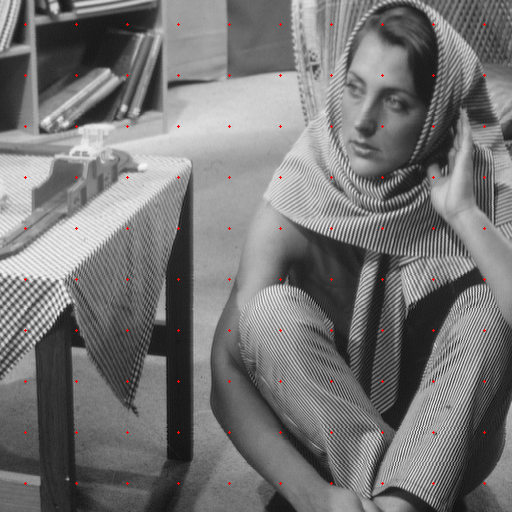
\includegraphics[width=0.6\textwidth]{img/spatiallyUniformSampling.png}
      \caption{Spatially uniform sampling. Red pixels are sampled. Here 100 pixels are sampled, which only represents 0.04\% of all pixels.}
  \end{figure}
 \item [Incremental sampling (INS)] is an adaptive sampling scheme, meaning that it select points according to the similarity, so that we can have an approximate optimal rank-k subspace of the original image \cite{zhan_improved_2017}.
 \item [Mean-shift segmentation-based sampling] this scheme performs good for complex backgrounds. The method consists in over-segmenting the image into \(n\) regions and only one pixel of each region will be sampled using the spatially closest pixel to the centre of the region given a formula in \cite{kao_sampling_2012}.
\end{description}

\subsection{Affinity function}
\label{variations:affinity_functions}

\paragraph{}
The kernel function measures the similarity between the pixel \(y_i\) and \(y_j\).
The chosen function is important because it decides on which features the similarity of pixels will be evaluated.
Some of the most used affinity functions are:

\begin{description}[align=left]
 \item [Spatial Gaussian Kernel] takes only into account the spatial distance between two pixels \cite{siam_slides_2016}.
  The formula of this kernel is, with \(\forall i, j \in [1, N]\), \(x_i\) the coordinate vector of a pixel and \(h_x\) a normalisation parameter,
  \[K(y_i, y_j) = exp(-\frac{||x_i - x_j||^2}{h_x^2}).\]
  The parameter is influencing on the normalisation of the values and Gaussian standard deviation.
  The greater it is, the more tolerant the spatial distance computation will be.

 \item [Photometric Gaussian Kernel] considers the intensity and colour similarity of the pixels \cite{siam_slides_2016}.
  The formula of this kernel is, with \(z_i\) the colour or grayscale of a pixel,
  \[K(y_i, y_j) = exp(-\frac{||z_i - z_j||^2}{h_z^2}).\]
  Generally, the \(h\) parameter is a smoothing parameter.
  If \(h\) is small, it is more discriminating between the affinity of different pixels.

 \item [Bilateral Kernel] one of the most used kernel which smooths images by a nonlinear combination of the spatial and photometric Gaussian kernels \cite{siam_slides_2016} \cite{glide_2014} \cite{bilateral_tomasi_1998}:
  \[K(y_i, y_j) = exp(-\frac{||x_i - x_j||^2}{h_x^2}) exp(-\frac{||z_i - z_j||^2}{h_z^2}).\]

  To generate the example below, we use the famous grayscale image of Barbara of size \(512 \times 512\) pixels.
  The more a pixel is coloured in red, the more similar it is to the selected pixel, with respect to the chosen bilateral kernel.
  A blue coloured pixel is dissimilar to the considered pixel.
  We use a spatially uniform sampling technique and select 0.1\% of the pixels.
  These are two affinity vectors; the first one is of a pixel on the table leg and the second around Barbara's eye.
  Keep in mind that each affinity image shown represents only one row of the affinity matrix\ \(K\).

  \begin{figure}[H]
      \centering
      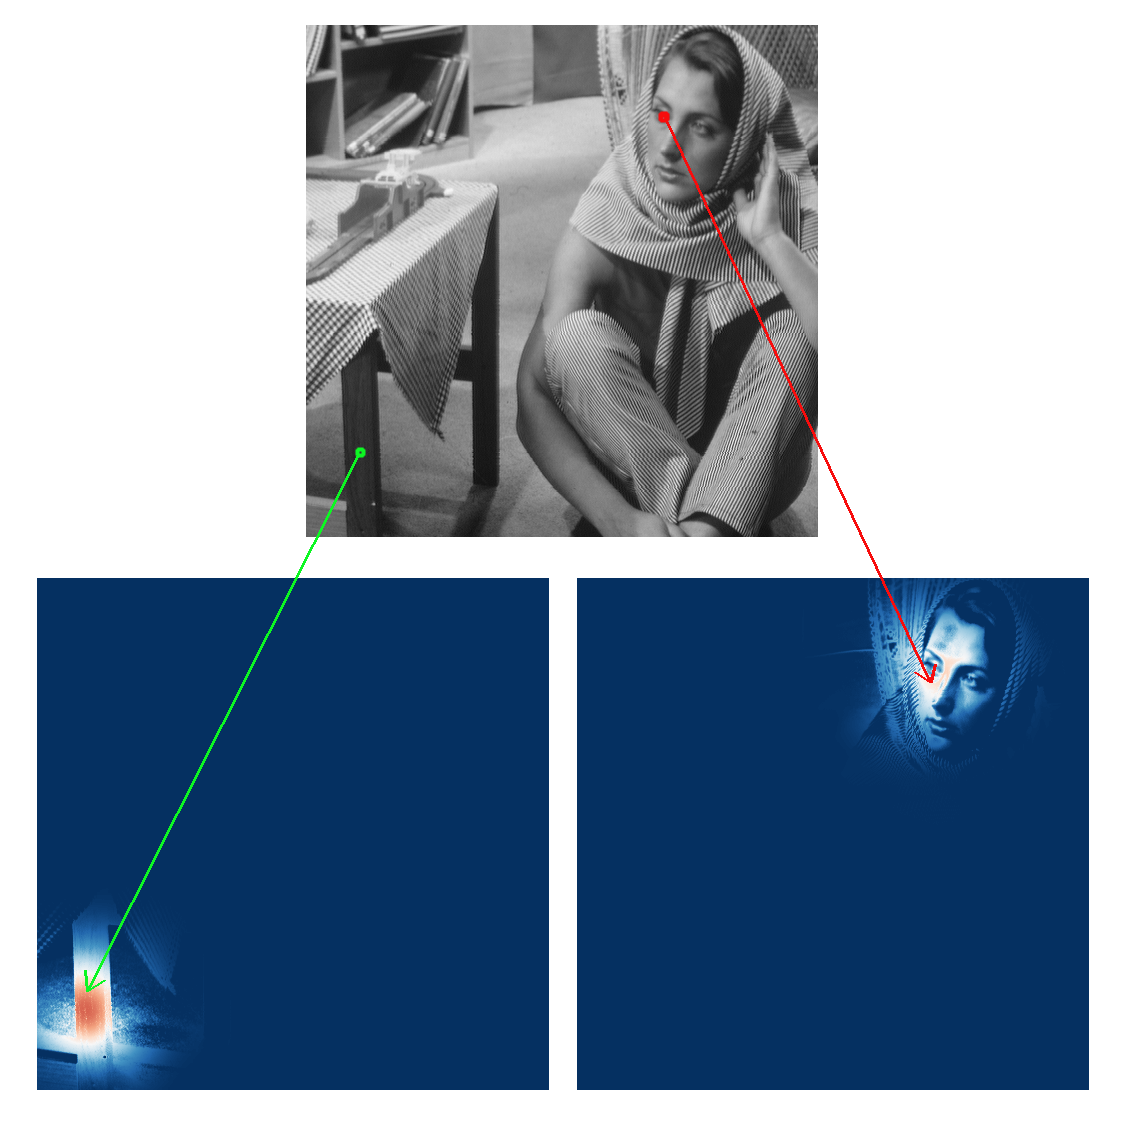
\includegraphics[width=\textwidth]{img/bilateralAffinityPhoto35Spatial50.png}
      \caption{Affinity matrices with \(h_x = 50\) and \(h_z = 35\).}
  \end{figure}
  In a very heterogeneous image, the bilateral kernel will be useful to keep the spatial similarity, but with excluding very dissimilar neighbour pixels.

 \item [Non-Local Means (NLM)] is similar to the bilateral kernel, a data-dependent filter, except that the photometric affinity is captured patch-wise \cite{glide_2014} \cite{kervrann_nlm_2006}.
 \item [Locally Adaptive Regression Kernel (LARK)] uses the geodesic distance based on estimated gradients \cite{milanfar_symmetrizing_2013} \cite{takeda_kernel_2007}.
\end{description}

\subsection{Graph Laplacian operator}

\paragraph{}
The graph Laplacian operator has multiple possible definitions and each has its own properties.
A good summary can be found in \cite{siam_slides_2016} and \cite{chung_spectral_1997}.
A graph Laplacian can be symmetric which is important for the eigendecomposition of the matrix.
The spectral range, corresponding to the range of the eigenvalues, is important because we can use the filters derived from the Laplacian multiple times, and if the eigenvalues are not between 0 and 1, then the filters tend to be unstable.
With \(K\) being the affinity matrix, \(d_i = \sum_j K_{ij}\) and \(D = diag\{d_i\}\):

\begin{table}[!htbp]
 \centering
 \begin{tabular}{|c|c|c|c|c|}
  \hline
  Laplacian Name & Formula of \(\Lapl\) & Symmetric & Spectral Range \\
  \hline
  Un-normalised & \(D - K\) & Yes & [0, n] \\
  \hline
  Normalised & \(I - D^{-1/2}KD^{-1/2}\) & Yes & [0, 2] \\
  \hline
  Random Walk & \(I - D^{-1}K\) & No & [0, 1] \\
  \hline
  ``Sinkhorn'' \cite{milanfar_symmetrizing_2013} & \(I - C^{-1/2}KC^{-1/2}\) & Yes & [0, 1] \\
  \hline
  Re-normalised \cite{milanfar_new_2016} & \(\alpha(D - K)\), \(\alpha = \bigO(N^{-1})\) & Yes & [0, n] \\
  \hline
 \end{tabular}
 \caption{Overview of different graph Laplacian operator definitions}
 \label{table:laplacians}
\end{table}
Generally, it is a good practice to stick to one definition of the Laplacian.
